\chapter{Theory}\label{sec:theory}

\section{The Standard Model}

The SM is currently our best theoretical framework for understanding the nature of fundamental particles. 
It is rooted in the idea that particles exist as excitations of quantum fields. These fields are constructed so as to obey 
fundamental symmetries of nature, and quantum field theory describes both the particles of our universe and their interactions. The SM is not only 
elegant and extensive, but provides a wide variety of measurable observables for the experimentalist to probe. So far, many 
measurements have been made of the known elementary particles and their interactions, and the predictions of the SM have held up in each case. In 
this respect, it is a wildly successful theory. In other respects, it is obviously incomplete. It does not account for the gravitational force, dark matter, or dark energy, among other phenomena. 
Thus, there is value in testing the SM even more carefully with experiments 
like those at the LHC, in hopes of refining our understanding and potentially discovering new physics. 

\section{The Elementary Particles} 

\begin{figure}[htb]
	\begin{center}
	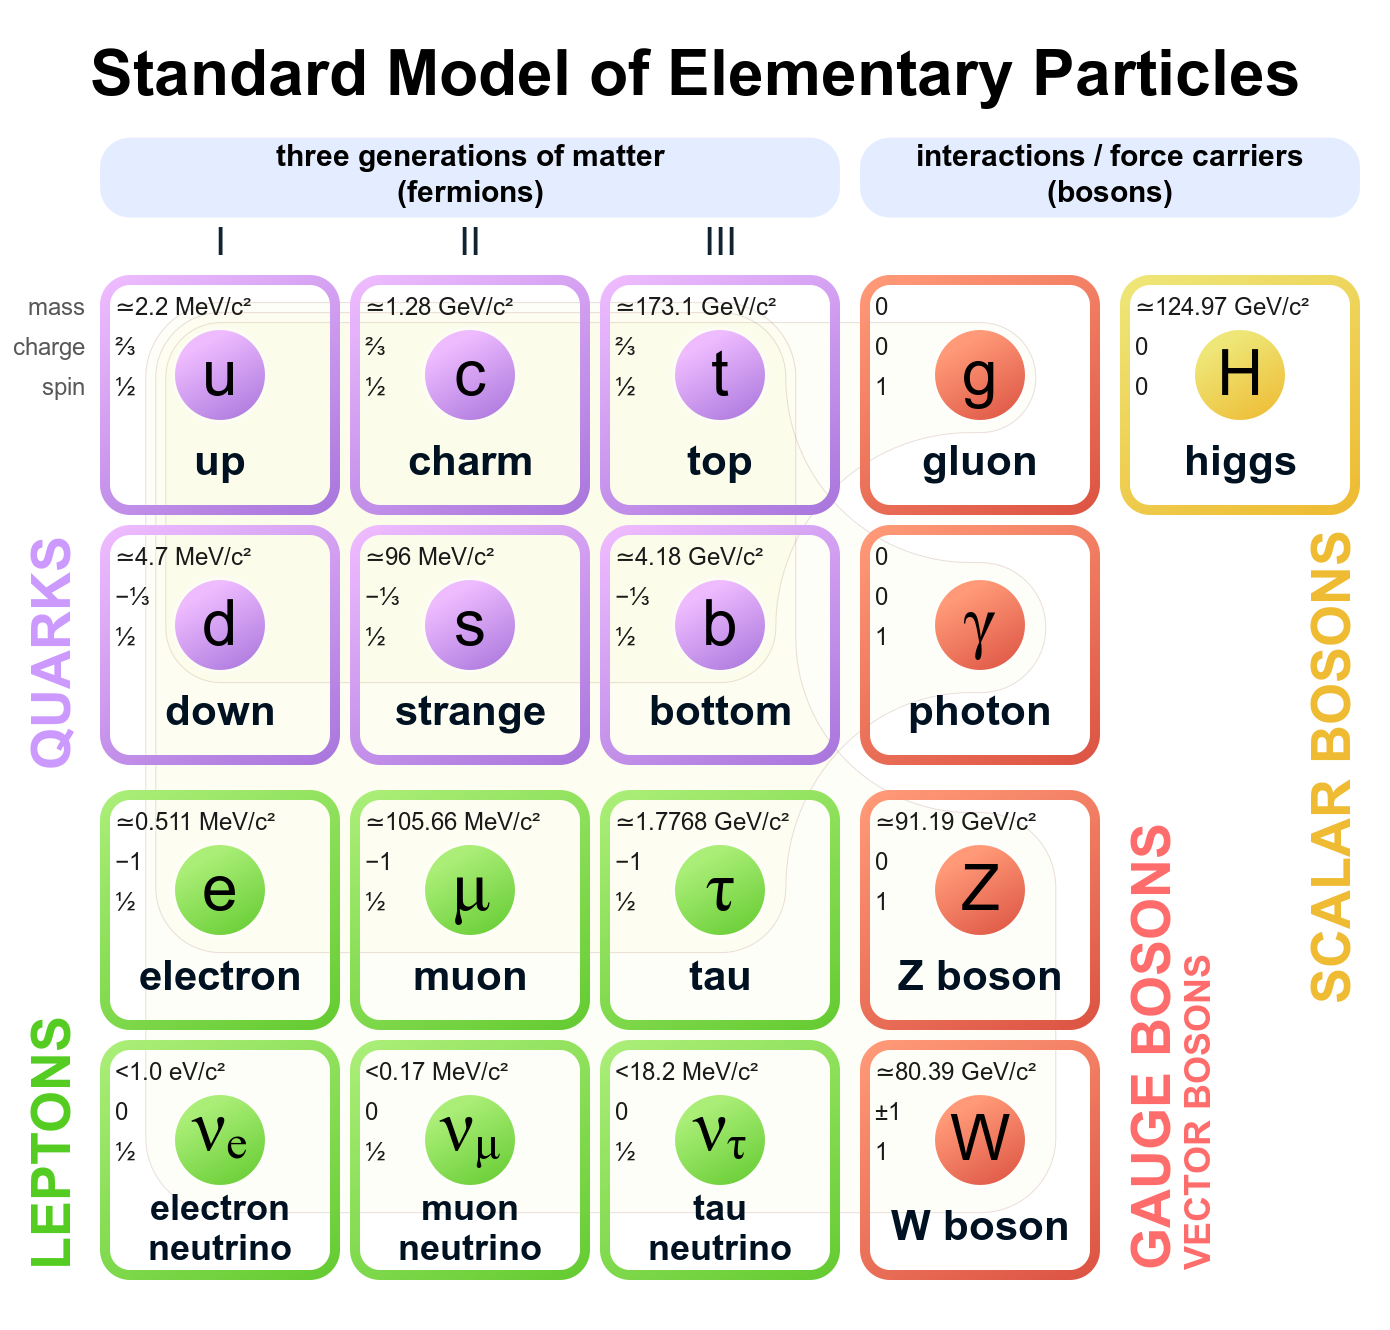
\includegraphics[width=0.65\textwidth]{fig/theory/Standard_Model_of_Elementary_Particles.png}
		\caption[Table of elementary particles in the SM. The leftmost three columns correspond to three generations of fermions, 
		the fourth column from the left shows the gauge bosons which mediate the elementary forces, and the rightmost column shows the Higgs boson. 
		For each particle, mass, charge, and spin are labeled, with mass values given as of 2019.]
		{Table~\cite{SMImage} of elementary particles in the SM. The leftmost three columns correspond to three generations of fermions, 
		the fourth column from the left shows the gauge bosons which mediate the fundamental forces, and the rightmost column shows the Higgs boson. 
		For each particle, mass, charge, and spin are labeled, with mass values given as of 2019.}
		\label{fig:SMParticles}
	\end{center}
\end{figure}

Figure \ref{fig:SMParticles} catalogs the elementary particles of the SM. These particles come in two broad types: fermions and bosons. Fermions are particles of half-integer spin that obey 
the Pauli exclusion principle. They are, therefore, responsible for the structure of matter. 
Each fermion has a corresponding antiparticle that has opposite electrical charge, but is otherwise identical. 
The fermions are subdivided into two types in three generations, the generations corresponding to mass.
Quarks are fermions that carry both fractional electric charge and color charge, so they participate in the electroweak and strong interactions. 
Leptons are fermions that carry integer electric charge and participate in the electroweak interaction.
In contrast to fermions, bosons have integer spin. The vector gauge bosons function as mediators of the fundamental forces of nature. 
The gluons mediate the strong force, the photon the electromagnetic force, and the W and Z bosons the weak force. 
Finally, the electrically neutral, scalar Higgs boson emerges due to electroweak symmetry breaking, described later in this section. The interaction of the Higgs 
with the other particles in the SM is responsible for particle masses. 
In the context of this thesis, which is a search for \hzg{}, the most relevant elementary particles are the Higgs boson, Z boson, leptons, and photon. 
Therefore, the remainder of this section will describe electroweak theory and the Higgs mechanism in more detail. Other aspects of the SM, such as quantum chromodynamics, 
are of importance in collider physics, but of less relevance for this specific search. Such topics are omitted in order to narrow the scope of the discussion.

\section{Electroweak Theory}
To motivate the Higgs mechanism and Higgs interactions, it is useful to first consider the electroweak interaction absent the Higgs. The electroweak piece of the 
SM Lagrangian can be written as 
\begin{align}
	& \mathcal{L}_{EW} = -\frac{1}{4}A_a^{\mu\nu}A^a_{\mu\nu} - \frac{1}{4}B^{\mu\nu}B_{\mu\nu} + i\sum_L \bar{L}\gamma^{\mu}D_{\mu,L}L + i\sum_R \bar{R}\gamma^{\mu}D_{\mu,R}R \label{eqn:LEWK}\\
	& A^a_{\mu\nu} = \partial_{\mu}A_{\nu}^{a} - \partial_{\nu}A_{\mu} + g\varepsilon_{abc}W^{b}_{\mu}W^{c}_{\nu} \\
	& B_{\mu\nu} = \partial_{\mu}B_{\nu} - \partial_{\nu}B_{\mu} \\
	& D_{\mu,L} = \partial_{\mu} + \frac{ig}{2}\tau\cdot A_{\mu} + \frac{ig'}{2}B_{\mu}Y \label{eqn:DL}\\
	& D_{\mu,R} = \partial_{\mu} + \frac{ig'}{2}B_{\mu}Y. \label{eqn:DR}
\end{align}
In the above equations, $A_{\mu\nu}^a$ represents an SU(2)$_L$ triplet of gauge fields and $B_{\mu\nu}$ represents a U(1) gauge field. The third and fourth terms in equation \ref{eqn:LEWK} 
describe the interactions of these gauge fields with the fermions, both quarks and leptons. Note that the interaction depends on the chirality of the fermions, where the left-handed 
fermions are denoted as $L$ and the right-handed as $R$. The right-handed fermions interact only with the U(1) field, while the left-handed fermions interact with the U(1) and SU(2)$_L$ fields. 
This is encoded by the derivative operators $D_{\mu,L}$ and $D_{\mu,R}$ defined in equations \ref{eqn:DL} and \ref{eqn:DR} in terms of the fields, Pauli matrices ($\tau$), hypercharge operator Y, and the couplings $g$ and $g'$. 

\section{Spontaneous Symmetry Breaking (Higgs Mechanism)}
One important property of the electroweak Lagrangian in equation \ref{eqn:LEWK} is that the bosons associated with the gauge fields are all massless. 
However, the direct observation of charged and neutral 
current interactions \cite{HASERT1973121,HASERT1973138} at CERN in 1973 implied that the W and Z boson must have relatively large masses in the range of 50--100\GeV. Indeed, the massive W and Z bosons were later discovered and measured \cite{UA1:1983crd,UA2:1983tsx} at the CERN Super Proton Synchroton in 1983. 
A solution to this shortcoming of the electroweak theory came in the form of the Higgs mechanism \cite{Englert:1964et,Higgs:1964ia,Higgs:1964pj},
which spontaneously breaks the SU(2)xU(1) gauge symmetry. One consequence of this is the addition of a real 
Higgs field accompanied by a massive Higgs boson. The W and Z boson masses arise naturally due to the electroweak symmetry breaking, 
while fermion masses are explained via additional Yukawa couplings to the Higgs boson. 
The discovery of the Higgs boson and subsequent measurements of its properties have provided experimental verification that the Higgs mechanism 
is a central piece of the Standard Model. 

To understand how the Higgs mechanism works, consider the introduction of a complex scalar field $\sf \Phi$, which 
transforms as a doublet under SU(2)$_L$.
\begin{equation}
    \label{eqn:higgsField}
    \Phi = 
    \begin{bmatrix}
        \phi^{+} \\ 
        \phi^{0}
    \end{bmatrix}
\end{equation}
Its contribution to the Lagrangian is given by:
\begin{equation}
    \mathcal{L_{H}} = (D^{\mu}_L\Phi)^{\dagger}(D_{\mu,L}\Phi) - V(\Phi)
    \label{LHiggs}
\end{equation}
where the Higgs potential takes the form
\begin{equation}
    V(\Phi) = \mu^{2}|\Phi^{\dagger}\Phi| + \lambda \Big(|\Phi^{\dagger}\Phi|\Big)^{2}.
    \label{VHiggs}
\end{equation}
Consider the case in which the parameters of the Higgs potential $\lambda$ and $\mu$ satisfy the conditions 
$\lambda > 0$ and $\mu^{2} < 0$. Then the shape of the potential is shown in Fig. \ref{fig:VHiggs} (right). There is no minimum of the 
potential at $\Phi = 0$. Rather, an infinite set of minima lie around a circle in the complex plane. Hence, it is said that $\Phi$ 
has a nonzero vacuum expectation value (VEV). The value of the VEV in terms of $\mu$ and $\lambda$ can be determined by explicitly
minimizing the potential:
\begin{align*}
    \frac{\partial}{\partial(\Phi^{\dagger}\Phi)}V(\Phi) &= 0 \\
    \mu^{2} + 2\lambda\Big(|\Phi^{\dagger}\Phi|\Big) &= 0 \\
    \mu^{2} + 2\lambda\Big[(\phi^{+})^{2} + (\phi^{0})^{2}\Big] &= 0 \numberthis
    \label{VHiggsMinimization}
\end{align*}
This can be minimized in many ways depending on individual values of $\phi^{+}$ and $\phi^{0}$ in the vacuum. By convention,
and without loss of generality, we choose the case in which $\phi^{+} = 0$. In this case we obtain the equation
\begin{equation}
    \phi^{0} = \sqrt{\frac{-\mu^{2}}{2\lambda}} = \frac{1}{\sqrt{2}}v
\end{equation}
where we have defined $v \equiv \sqrt{-\mu^{2}/\lambda}$.

\begin{figure}
	\begin{center}
	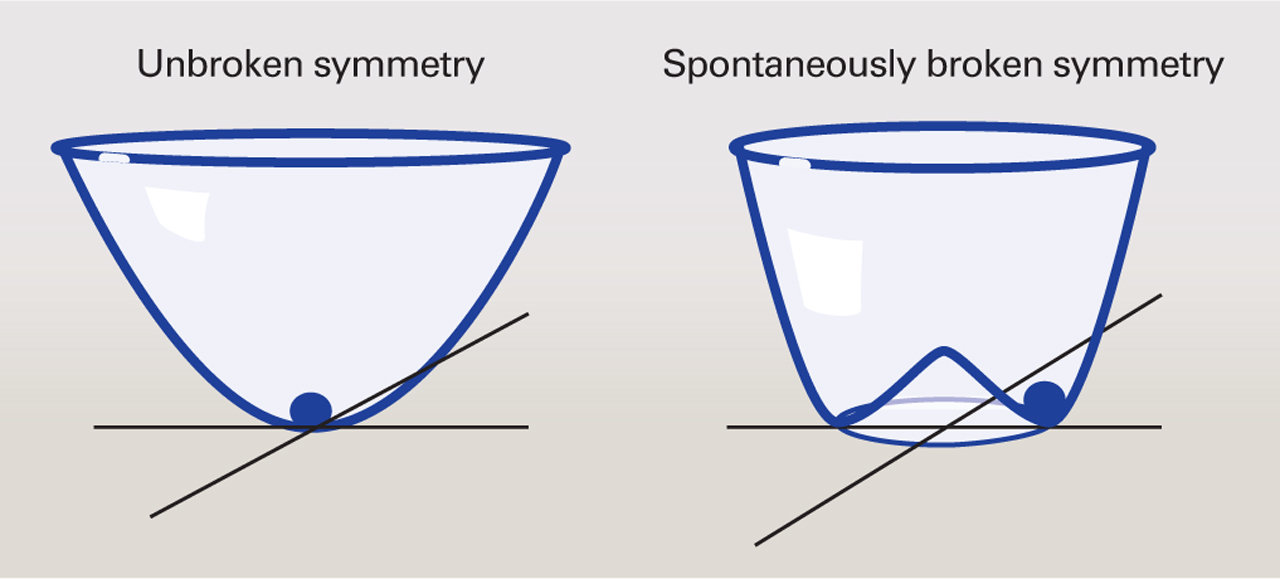
\includegraphics[width=0.75\textwidth]{fig/theory/spont_sym_breaking.jpg}
		\caption
		[Comparison of the shapes of complex scalar potentials without symmetry breaking (left) and with spontaneous symmetry breaking (right). 
		The transverse axes represent the real-imaginary $\Phi$ plane, 
		and the vertical axis represents the magnitude of the potential $V(\Phi)$. The diagram at right corresponds to the shape of the Higgs potential in the SM.]
		{Comparison of the shapes of complex scalar potentials without symmetry breaking (left) and with spontaneous symmetry breaking (right)~\cite{VHiggsImage}. 
		The transverse axes represent the real-imaginary $\Phi$ plane, 
		and the vertical axis represents the magnitude of the potential $V(\Phi)$. The diagram at right corresponds to the shape of the Higgs potential in the SM.}
		\label{fig:VHiggs}
	\end{center}
\end{figure}

The existence of the Higgs VEV has profound implications. To see this, it is helpful to reparameterize the scalar doublet field
$\Phi$ as follows:
\begin{equation}
    \Phi = \frac{1}{\sqrt{2}}e^{i\frac{\tau^{a}}{2}\theta_{a}(x)}
    \begin{bmatrix}
        0 \\
        v + h(x)
    \end{bmatrix}
    \label{reparamHiggsField}
\end{equation}
As $\Phi$ is invariant under local SU(2)$_L$ gauge transformations, the prefactor may be rotated away. This is equivalent to setting 
$\theta(x) = 0$ in equation \ref{reparamHiggsField}. This choice of gauge is known as the unitary gauge, and leads to 
\begin{equation}
    \Phi = \frac{1}{\sqrt{2}}
    \begin{bmatrix}
        0 \\
        v + h(x)
    \end{bmatrix}
    \label{HiggsFieldUnitaryGauge}
\end{equation}
Given the above form of $\Phi$, we can now evaluate the Higgs Lagrangian (equation \ref{LHiggs}), starting with the kinetic term
$(D^{\mu}_L\Phi)^{\dagger}(D_{\mu,L}\Phi)$.
\begin{align*}
    (D^{\mu}_L\Phi)^{\dagger}(D_{\mu,L}\Phi) &= \Big| (\partial_{\mu} - \frac{ig}{2}\tau\cdot A_{\mu} - \frac{ig'}{2}B_{\mu}Y)\Phi\Big|^{2} \\
    &= \frac{1}{2}
    \Big| 
    \begin{bmatrix}
        \partial_{\mu} - \frac{i}{2}(gA_{\mu}^{3} + g'B_{\mu}) & -\frac{ig}{2}(A_{\mu}^{1} - iA_{\mu}^{2}) \\
            -\frac{ig}{2}(A_{\mu}^{1} + iA_{\mu}^{2}) & \partial_{\mu} + \frac{i}{2}(gA_{\mu}^{3} - g'B_{\mu})
    \end{bmatrix} 
    \begin{bmatrix}
        0 \\ 
        v + h(x)
    \end{bmatrix} 
    \Big|^{2} \\ &=  
    \frac{1}{2}\Big| 
    \begin{bmatrix}
        -\frac{ig}{2}(A_{\mu}^{1} - iA_{\mu}^{2})(v + h(x)) \\
        \partial_{\mu}h(x) + \frac{i}{2}(gA_{\mu}^{3} - g'B_{\mu})(v + h(x))
    \end{bmatrix}
    \Big|^{2} \\ &= 
    \frac{1}{2}\partial_{\mu}h(x)\partial^{\mu}h(x) + \frac{1}{8}(gA_{\mu}^{3} - g'B_{\mu})(gA^{\mu}_{3} - g'B^{\mu})(v + h(x))^{2} \\ &+ 
    \frac{g^{2}}{8}(A_{\mu}^{1} - iA_{\mu}^{2})(A_{\mu}^{1} + iA_{\mu}^{2})(v + h(x))^{2} \label{kinHiggsExpansion} \numberthis 
\end{align*}
With some foreknowledge of the result, we define the physical gauge fields and their masses.
\begin{align}
    W_{\mu}^{\pm} &= \frac{1}{\sqrt{2}}(A_{\mu}^{1} \mp iA_{\mu}^{2}) \; &m_{W} = \frac{gv}{2} \\
    Z_{\mu} &= \frac{1}{\sqrt{g^{2} + g'^{2}}}(gA_{\mu}^{3} - g'B_{\mu}) \; &m_{Z} = \sqrt{g^{2} + g'^{2}}\frac{v}{2} \\
    A_{\mu} &= \frac{1}{\sqrt{g^{2} + g'^{2}}}(g'A_{\mu}^{3} + gB_{\mu}) \; &m_{A} = 0
    \label{gaugeBosonsAndMasses}
\end{align}
Then the kinetic term of the Higgs Lagrangian can be recast as
\begin{align*}
    (D^{\mu}_L\Phi)^{\dagger}(D_{\mu,L}\Phi) &= \frac{1}{2}\partial_{\mu}h(x)\partial^{\mu}h(x) \\ 
    &+ \frac{1}{2}m_{Z}^{2}Z_{\mu}Z^{\mu} + m_{W}^{2}W_{\mu}^{+}W^{-\mu} \\
    &+ \frac{v}{4}(g^{2} + g'^{2})Z_{\mu}Z^{\mu}h + \frac{1}{8}(g^{2} + g'^{2})Z_{\mu}Z^{\mu}h^{2} \\
    &+ \frac{v}{4}g^{2}W_{\mu}^{+}W^{-\mu}h + \frac{1}{8}g^{2}W_{\mu}^{+}W^{-\mu}h^{2} \label{kinHiggsMasses}\numberthis
\end{align*}
Equation \ref{kinHiggsMasses} provides a great deal of information on the physical ramifications of the Higgs mechanism.
The first term is the kinetic term of the physical Higgs boson field. The second and third terms are the mass terms of the Z and W 
bosons, respectively. The fourth and fifth terms show the linear and quadratic couplings of the Z boson to the Higgs boson, respectively.
Finally, the sixth and seventh terms show the linear and quadratic couplings of the W boson to the Higgs boson, respectively. 
Given the form of equation \ref{HiggsFieldUnitaryGauge}, a similar expansion can be carried out on the Higgs potential
(equation \ref{VHiggs}). Here, the terms involving the physical Higgs boson are most interesting, so constant terms are dropped.
\begin{align*}
    V(\Phi) &= \frac{\mu^{2}}{2}(v+h)^{2} + \frac{\lambda}{4}((v+h)^{2})^{2} \\
    &\rightarrow \lambda v^{2}h^{2} + \lambda vh^{3} + \frac{\lambda}{4}h^{4} \label{expandedVHiggs} \numberthis
\end{align*}
The first term is a Higgs mass term, with $m_{H} = \sqrt{2\lambda v^{2}}$. The second and third terms describe the Higgs 
trilinear and quartic self-couplings, respectively.

The Lagrangian including the Higgs doublet $\Phi$ can be further extended to incorporate interactions between the Higgs and fermion fields. These interactions, along with the nonzero Higgs VEV, provide a mechanism to generate the fermion masses. The interactions take the 
form of Yukawa couplings:
\begin{equation}
    \mathcal{L}_{Yukawa} = Y_{ij}^{d}\bar{Q}^{i}_{L}\Phi d_{R}^{j} + Y_{ij}^{u}\bar{Q}^{i}_{L}\tilde{\Phi} u_{R}^{j} 
    + Y_{ij}^{e}\bar{L}^{i}_{L}\Phi e_{R}^{j} + h.c.,
    \label{LYukawa}
\end{equation}
where $\tilde{\Phi} \equiv i\tau_{2}\Phi^{*}$, and $u$, $d$, and $e$ represent up-type quarks, down-type quarks, and leptons, respectively. The constants $Y_{ij}^a$ denote the Yukawa couplings in each case, $Q^i$ is the set of SU(2) quark doublets, and $L^i$ is the set of SU(2) lepton doublets.
\begin{equation}
    \tilde{\Phi} \equiv i\tau_{2}\Phi^{*}
    \label{PhiDual}
\end{equation}
Plugging in the unitary gauge parameterization of equation \ref{HiggsFieldUnitaryGauge}, this evaluates to 
\begin{align}
    \mathcal{L}_{Yukawa} = \frac{Y_{ij}^{d}}{\sqrt{2}}\bar{d}_{L}^{i}(v + h)d_{R}^{j} 
    + \frac{Y_{ij}^{u}}{\sqrt{2}}\bar{u}_{L}^{i}(v+h)u_{R}^{j} + \frac{Y_{ij}^{e}}{\sqrt{2}}\bar{e}_{L}^{i}(v+h)e_{R}^{j}
    \label{expandedLYuk}
\end{align}
It is worth looking closely at the terms in equation \ref{expandedLYuk}. For a given fermion type, the first term in the parentheses
is a fermion mass term. The second term in the parentheses gives the coupling of the fermion to the Higgs boson. With this in mind, 
we observe that the fermion mass is given in terms of the couplings and the Higgs vev by 
\begin{equation}
    m_{f} = \frac{y_{f}v}{\sqrt{2}}
    \label{fermionMass}
\end{equation}
where $y_{f}$ is the relevant value taken from the Yukawa coupling matrix. In addition, we see that the strength of the fermion coupling
to the Higgs boson is given by $\frac{m_{f}}{v}$. Thus, fermions couple to the Higgs boson with strength directly proportional 
to their masses. This result has important consequences in the context of collider experiments, as it regulates the rates of
Higgs production and decay related to each fermion-Higgs interaction. 

%The existence of the Higgs VEV leads naturally to the masses of the W and Z bosons. This can be shown by squaring the covariant 
%derivative acting on the scalar doublet $\Phi$ and evaluating the result in the vacuum. Note that in the vacuum, all terms involving 
%the partial derivative $\partial_{\mu}$ will yield zero contribution. Therefore, keeping only the relevant terms, the squared covariant 
%derivative reduces to
%\begin{equation}
%    |D_{\mu}|^{2} \rightarrow (\frac{g}{2}A_{\mu}^{a}\tau^{a} +\frac{g'}{2}B_{\mu})(\frac{g}{2}A^{b\mu}\tau^{b} + \frac{g'}{2}B^{\mu})
%    \label{covDerivSquared}
%\end{equation}
%Evaluating this in the vacuum yields
%\begin{align}
%    \Delta\mathcal{L} &= \frac{1}{2}
%    \begin{bmatrix}0 & v
%    \end{bmatrix}
%    (\frac{g}{2}A_{\mu}^{a}\tau^{a} +\frac{g'}{2}B_{\mu})(\frac{g}{2}A^{b\mu}\tau^{b} + \frac{g'}{2}B^{\mu}) 
%    \begin{bmatrix}
%        0 \\ 
%        v
%    \end{bmatrix} \\ 
%    \Delta\mathcal{L} &=
%    \frac{1}{2}\frac{v^{2}}{4}[g^{2}(A_{\mu}^{1})^{2} g^{2}(A_{\mu}^{2})^{2} + (g'B_{\mu} - gA_{\mu}^{3})^{2}]
%\end{align}
%From this, we can identify the fields and masses for the positively and negatively charged W bosons and the neutral Z boson and photon. 
%These are as follows:


\section{Higgs Production}

At a hadron collider like the LHC, the Higgs boson can be produced via several different mechanisms, each mechanism occuring at a certain rate. The dominant production 
mechanism is gluon-gluon fusion (ggH), followed by vector boson fusion (VBF) production, which is about an order of magnitude rarer. Less common production mechanisms, but 
still relevant for a search at the LHC, are the associated production mechanisms WH, ZH, and t$\bar{t}$H. The cross sections for each Higgs production mechanism as a function of 
center of mass energy are shown in Fig. \ref{fig:higgs_prod}.

\begin{figure}
	\begin{center}
	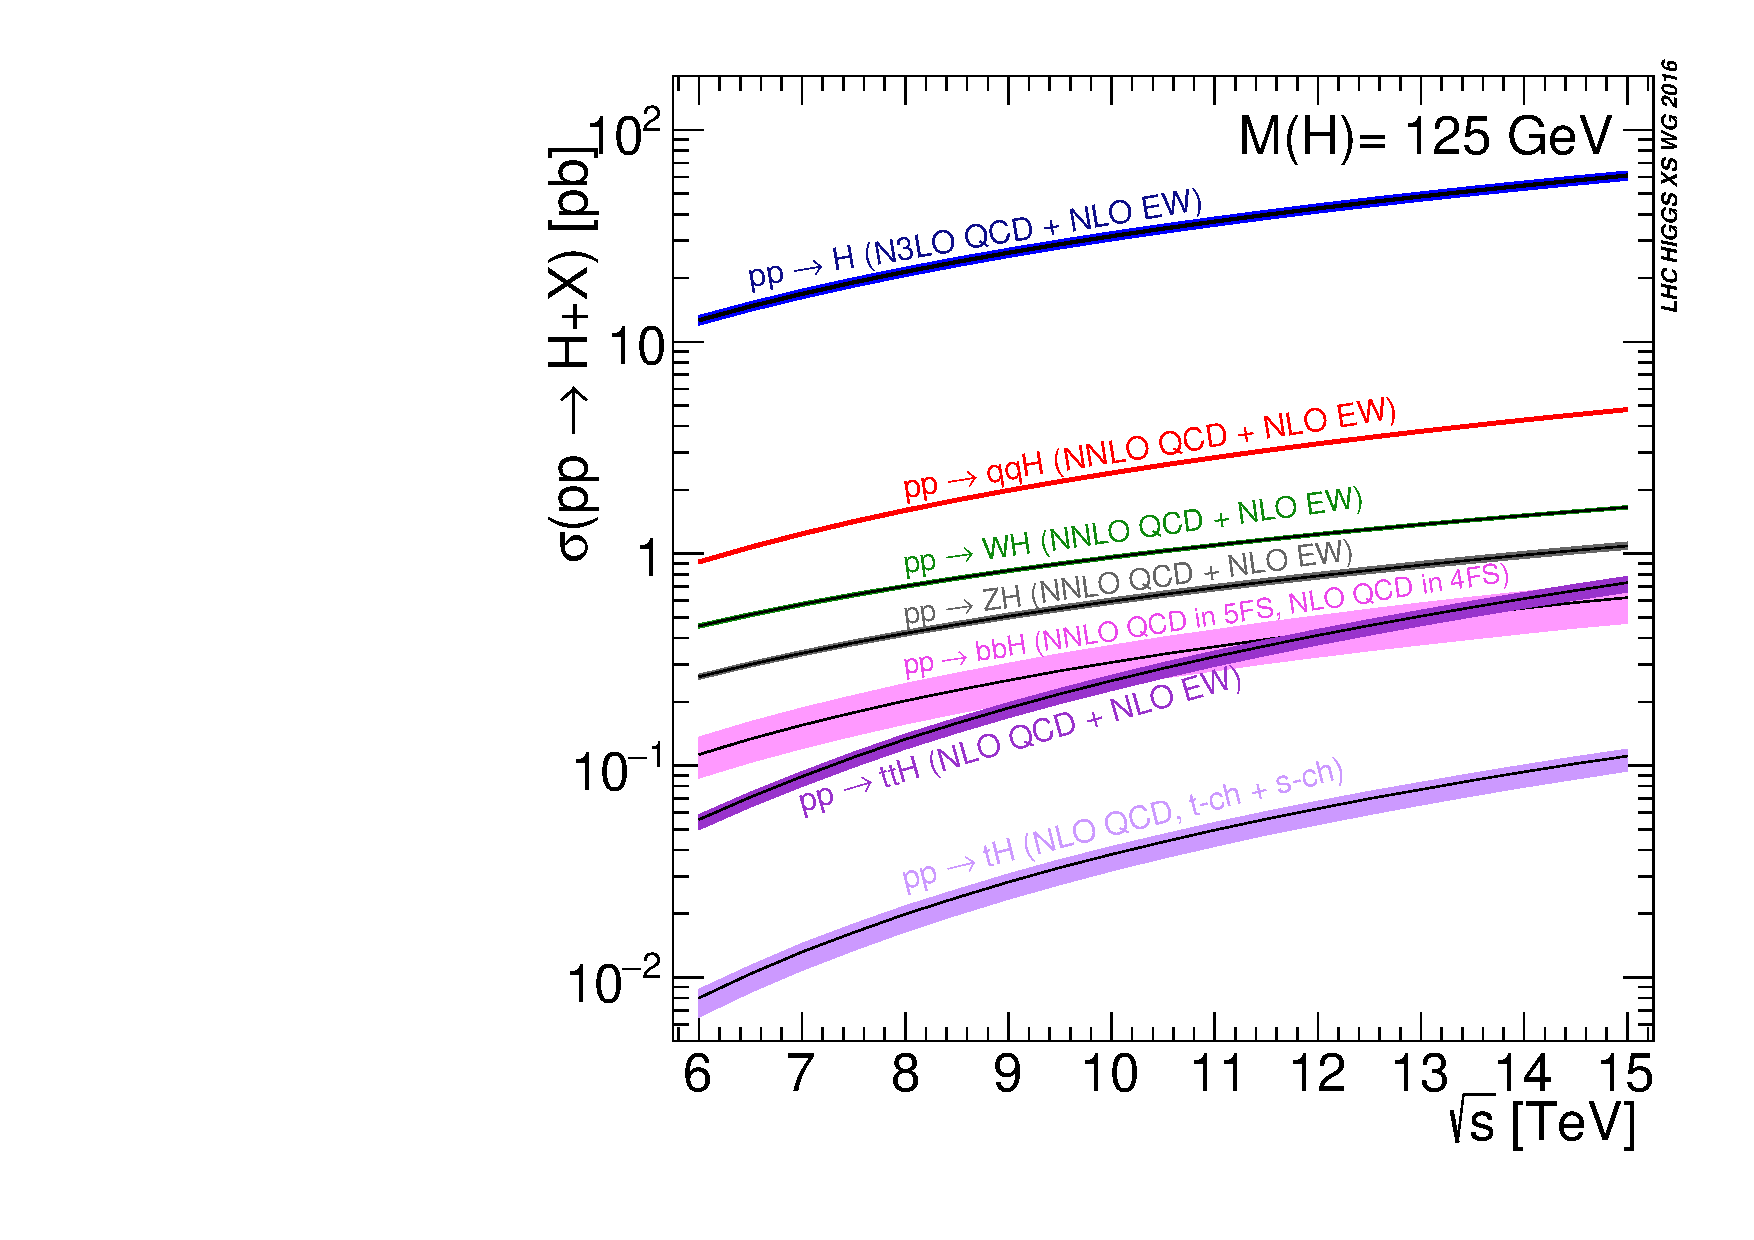
\includegraphics[width=0.75\textwidth]{fig/theory/Plot_Escan_H125_new_sqrt.pdf}
	\caption{Cross sections for different Higgs boson production mechanisms as a function of center of mass energy.}
	\label{fig:higgs_prod}
	\end{center}
\end{figure}

\section{Higgs Decay}

The Higgs boson decays rapidly after it is produced at the LHC. It can decay into a variety of final states, each occuring at a certain rate. Tree-level Higgs decays occur at rates 
proportional to the square of the mass of the decay products. Decays to b$\bar{b}$, WW, $\tau^+\tau^-$, and ZZ, are among the most common and experimentally accessible at the LHC. Other Higgs decays 
occur at loop-level, including $\PH \to \Pg\Pg$ and \hzg. Figure \ref{fig:higgs_br} shows the branching fractions at $\sqrt{s}=13$\TeV for different decay channels as a function of Higgs boson mass. 
We see that the branching fraction of \hzg is suppressed relative to several other production modes, so a search for \hzg must rely on the clean $\ell^+\ell^-\gamma$ signature.

\begin{figure}
	\begin{center}
	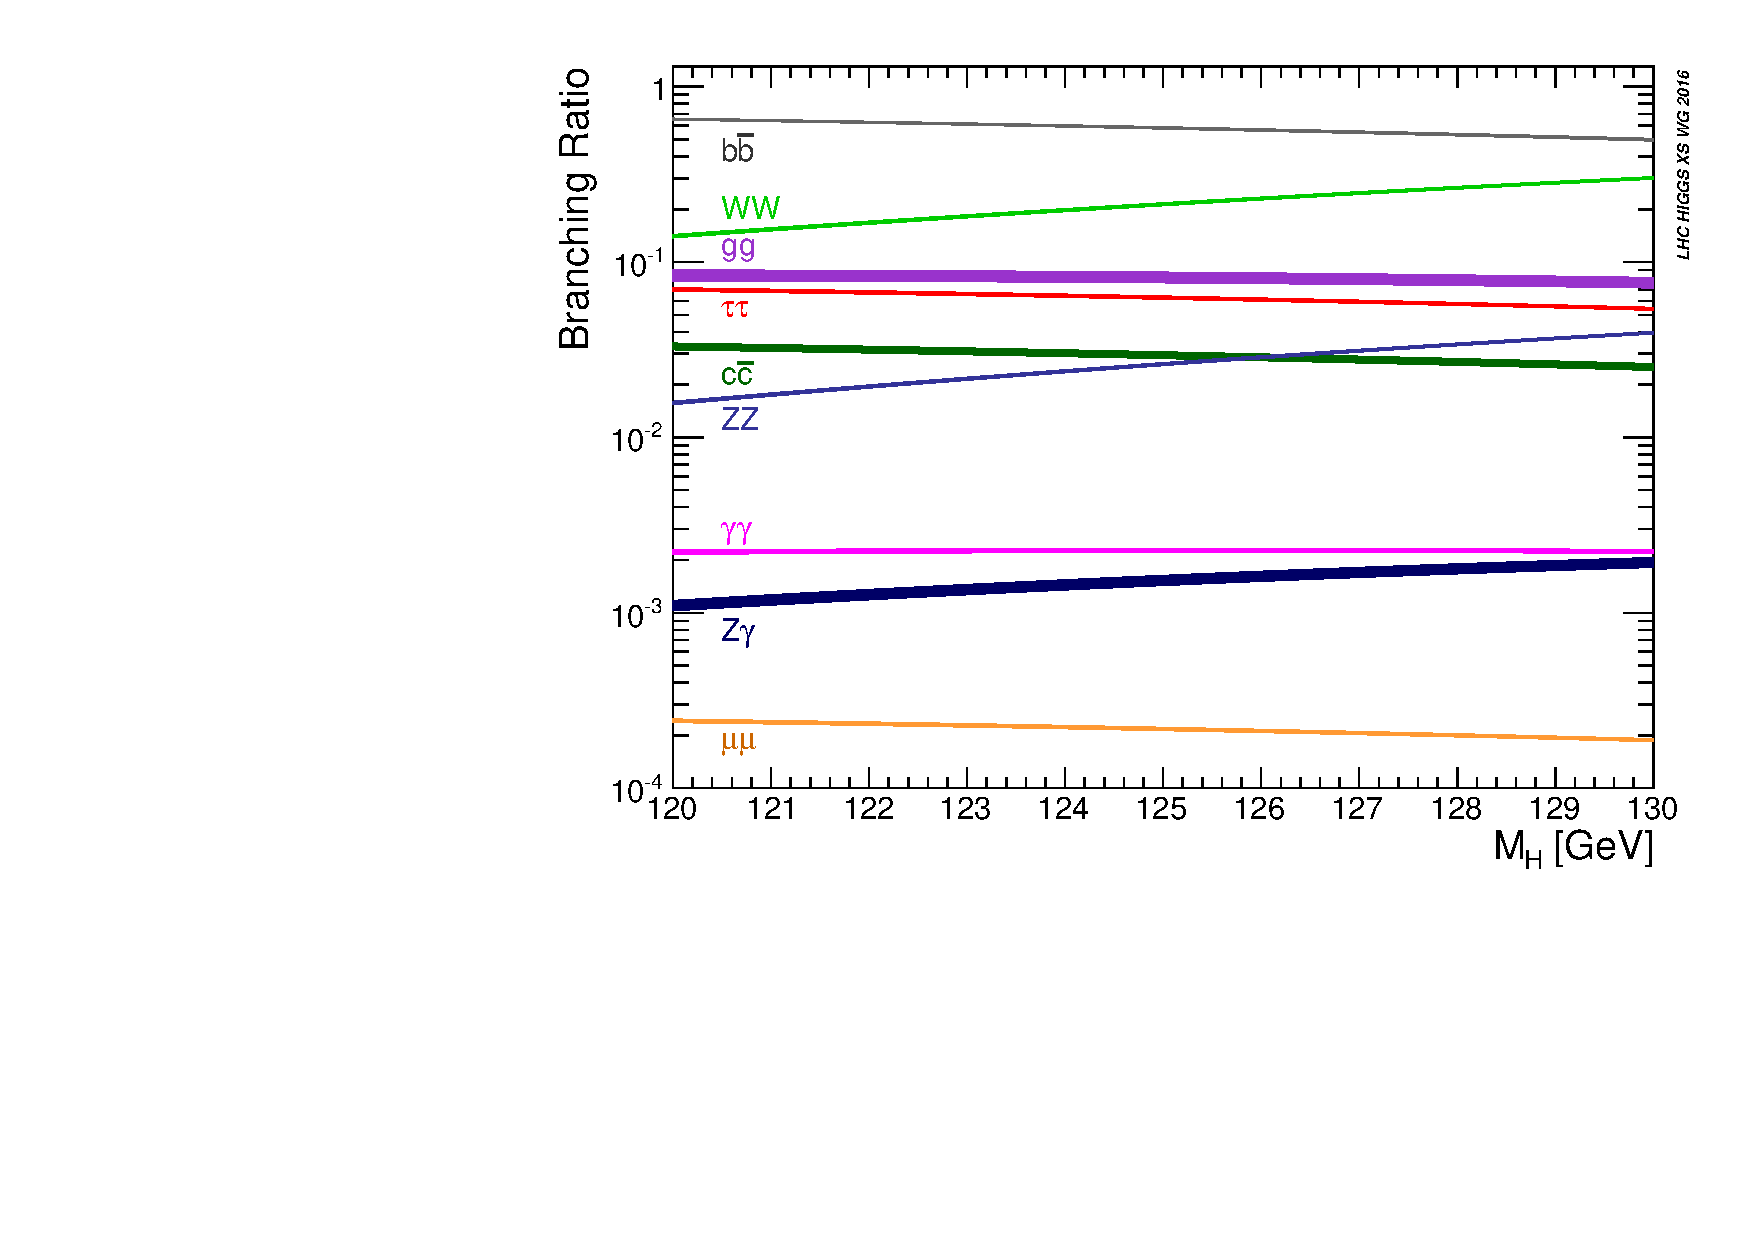
\includegraphics[width=0.75\textwidth]{fig/theory/SMHiggsBR.YR4-rect.pdf}
		\caption{Branching fraction of \hzg decay as a function of Higgs boson mass.}
		\label{fig:higgs_br}
	\end{center}
\end{figure}

\section{Physics Beyond the Standard Model}

One of the goals of the LHC is to search for BSM physics. While the decay \hzg{} is predicted in the SM, searching for it and measuring its branching fraction can indirectly probe potential 
new physics phenomena. A few unique features of \hzg{} make it well-suited as a BSM probe. First, the decay is loop-induced, which means that the introduction of new particles will contribute 
to the loop, interfering and altering the final branching fraction. Secondly, the decay \hgg{} is a very similar loop-induced process that has been discovered and measured extensively 
by the CMS and ATLAS Collaborations [REFS]. This means any new particle content entering into the \hzg{} loop will also enter into the \hgg{} loop. However, in the case of \hzg{}, the
Z boson couples to loop particles according to the SU(2)xU(1) quantum number rather than just the electric charge, as is the case for \hgg{}. 
It follows that potential BSM physics scenarios can shift the 
branching fractions of \hzg{} and \hgg{} by differing amounts, making the ratio $\mathcal{B}(\PH\rightarrow\PZ\gamma)/\mathcal{B}(\PH\rightarrow\gamma\gamma)$ a sensitive observable. In the SM, 
$\mathcal{B}(\PH\rightarrow\PZ\gamma)/\mathcal{B}(\PH\rightarrow\gamma\gamma) = 0.69 \pm 0.04$. A measurement of a significant deviation from this value would be an indicator of possible BSM physics.
Below, we describe a few examples of BSM scenarios that can affect this ratio.

One way to consider BSM effects in the context of \hzg{} is to introduce new particles, like a W' boson, charged scalar, or a pair of charged leptons. 
This is the approach taken by Carena, Low, and Wagner~\cite{Zg_theory_decaywidth}. The W' possibility is motivated by the fact that the W boson loop is the dominant 
contribution in the SM. The W' can be defined by an SU(2) triplet and characterized by mass and Higgs coupling parameters. Figure \ref{fig:rzg_bsm} (left) shows contours of constant branching fraction 
enhancement in the \hzg{} and \hgg{} decay channels in the mass-coupling plane for the W' model. 
Depending on the parameter values, the level of enhancement can be up to double the SM value, and it differs 
significantly in the two channels. Similarly, we can imagine a new charged scalar or a pair of new charged leptons. The branching fraction enhancement contour plots in Fig. \ref{fig:rzg_bsm} show that for similar regions in the mass-coupling plane, \hzg{} can be enhanced, while \hgg{} is simultaneously diminished. 

Other relevant BSM physics models include extended Higgs sectors. Such models often contain charged Higgs bosons, which enter into the \hzg{} and \hgg{} loops and impact the branching fractions. 
In Ref. \cite{Zg_theory_extension}, Chiang and Yagyu catalog extended Higgs models of varying types: models with one singly-charged boson, those with one singly-charged and one doubly-charged boson, 
and those with two singly-charged bosons. In total, the authors consider thirteen models, including the two Higgs doublet model, the minimal SUSY model, and the Higgs triplet model. 
Figure \ref{fig:exthiggs} gives the ratio of decay widths $\Gamma(\PH\rightarrow\PZ\gamma)/\Gamma(\PH\rightarrow\gamma\gamma)$ as a function of the mass coefficient of the additional scalar field(s) for seven of the models. It is evident that, for mass scales accessible at the LHC, the ratio can be significantly shifted relative to the SM expectation. 


\begin{figure}[tb]
	\begin{center}
		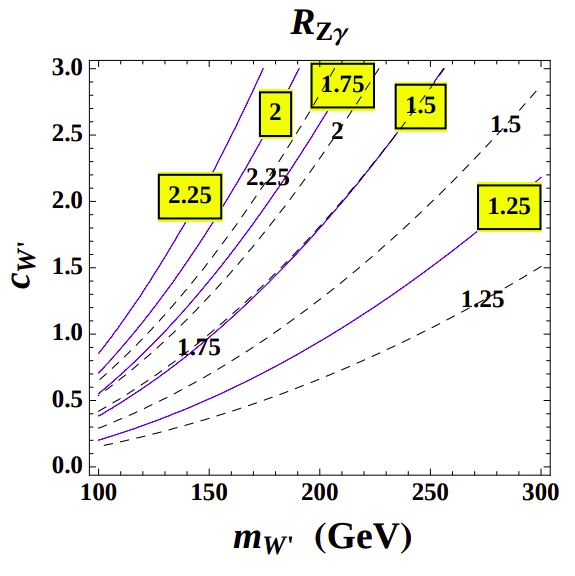
\includegraphics[width=0.30\textwidth, height=.30\textwidth]{fig/theory/rzgamma_wprime.png}
		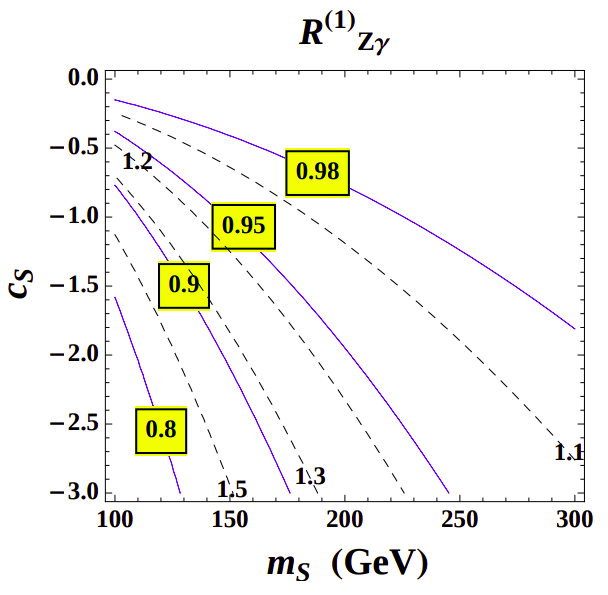
\includegraphics[width=0.30\textwidth, height=.30\textwidth]{fig/theory/rzgamma_scalar.png}
		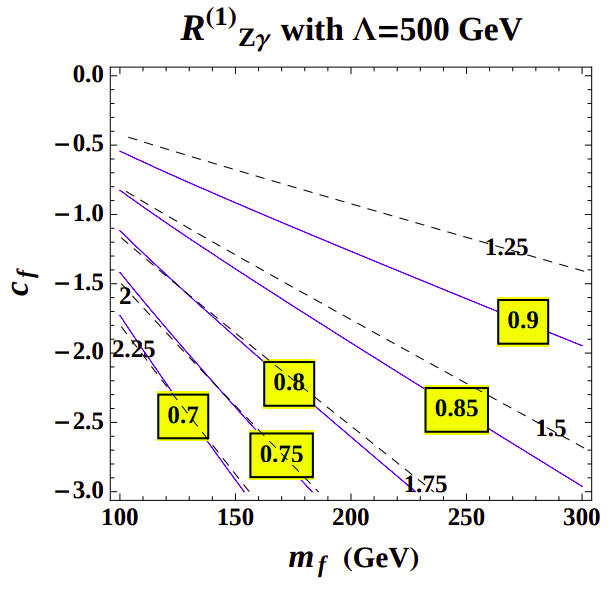
\includegraphics[width=0.30\textwidth, height=.30\textwidth]{fig/theory/rzgamma_fermion.png}
		\caption[Contours of constant branching fraction enhancement relative to the SM for the W' (left), charged scalar (center), 
		and charged lepton (right) scenarios. 
		The solid lines represent contours of enhancement in $\mathcal{B}$(\hzg), while the dashed lines correspond to \hgg{}. The yellow boxed numbers label the enhancement for each 
		\hzg{} contour, and the unboxed numbers label the enhancement for each \hgg{} contour.]
		{Contours of constant branching fraction enhancement relative to the SM for the W' (left), charged scalar (center), 
		and charged lepton (right) scenarios~\cite{Zg_theory_decaywidth}. 
		The solid lines represent contours of enhancement in $\mathcal{B}$(\hzg), while the dashed lines correspond to \hgg{}. The yellow boxed numbers label the enhancement for each 
		\hzg{} contour, and the unboxed numbers label the enhancement for each \hgg{} contour.}
		\label{fig:rzg_bsm}
	\end{center}
\end{figure}

\begin{figure}[tb]
	\begin{center}
		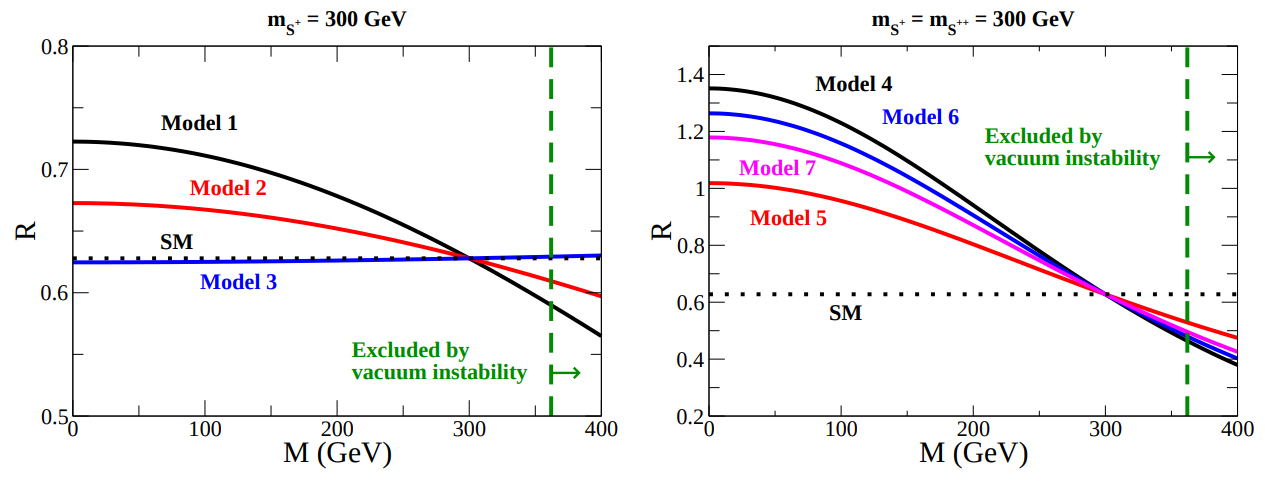
\includegraphics[width=0.9\textwidth]{fig/theory/rzgamma_exthiggs.png}
		\caption[Ratio of decay widths $\Gamma(\PH\rightarrow\PZ\gamma)/\Gamma(\PH\rightarrow\gamma\gamma)$ as a function of the mass coefficient of the additional scalar field(s) for 
		seven BSM models with extended Higgs sectors. 
		The models plotted on the left correspond to one additional singly-charged boson, and those on the right to one additional singly-charged and one additional doubly-charged boson.]
		{Ratio of decay widths $\Gamma(\PH\rightarrow\PZ\gamma)/\Gamma(\PH\rightarrow\gamma\gamma)$ as a function of the mass coefficient of the additional scalar field(s) for 
		seven BSM models with extended Higgs sectors~\cite{Zg_theory_extension}. 
		The models plotted on the left correspond to one additional singly-charged boson, and those on the right to one additional singly-charged and one additional doubly-charged boson.}
		\label{fig:exthiggs}
	\end{center}
\end{figure}
